\begingroup
% Prevent new pages between chapters (in group)
\let\clearpage\relax
\chapter{Introduction}

Three attributes of a secure system (\textblue{CIA}) :
\begin{itemize}
    \item \textblue{Confidentiality} : Cant read/steal data
    \item \textblue{Integrity} : Cant modify data
    \item \textblue{Availability} : Cant distrub access to data
\end{itemize}

\chapter{Access Control}

Access control is about the Confidentiality and Integrity. The goal is to restrict the access to a resource to authorized users only.
This resource can be data or CPU (analogy : steal server resources for mining).
\begin{itemize}
    \item \textblue{Principle of least privileges} : Define the access control rules such that users only have those access rights that they need to do their job (e.g. User "Peter" can access /home/peter but not /home/mary)
    \item \textblue{Implementing access control} : Identify verification via login, unix file permissions, Access Control Lists (ACL), ...
    \item \textblue{Breaking access control} : Physical (steal computer), Social engineering (convince a lgeitimate user to five the resource/access right to you), ...
\end{itemize}

\chapter{How a CPU executes programs}

Each running process gets its own virtual address space. When the program is loaded, the OS reserves blocks in main memory. It contains :
\begin{itemize}
    \item \textblue{TEXT} segment (Code of the program)
    \item \textblue{DATA} segment (Constants, ...)
    \item \textblue{HEAP} segment (Dynamically loaded librearies (\ctext{lightGray}{.dll/.so})) : Grows by allocation \textit{manually} memory space (e.g. with \ctext{lightGray}{malloc})
    \item \textblue{STACK} segment (Variables values, ...) : Grow downwards by allocating \textit{automatically} (via 
\end{itemize}

A CPU has several \textblue{registers} (temporary data stores that are used to perform calculations). For the CPU, variables are just locations in main memory. There is a special register that contains the address of the next instruction to be executed, called the \textblue{Instruction Pointer (ip)} (or Program Counter (pc)). Another register, the \textblue{Stack Pointer (sp)} contains the top of the stack's address.

When a function is called, a stack fram eis put on the stack during runtime. When $f(3, 4)$ returns, the top stack frame is removed from the stack, and the program exection continues at the instruction stored at the return address. Many CPUs have a \textblue{framepointer register (fp)} that points at the end of the block with local variables, that allows to easily calculate the address of its local variables and parameters.

\begin{figure}[H]
    \centering
    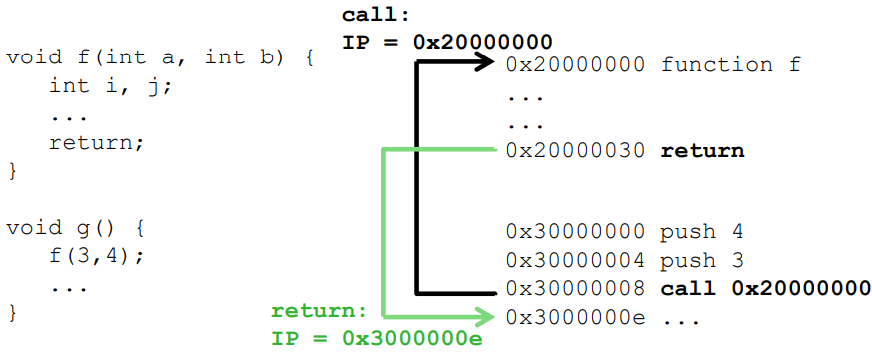
\includegraphics[width=0.55\textwidth,keepaspectratio]{function_call}\hfill
	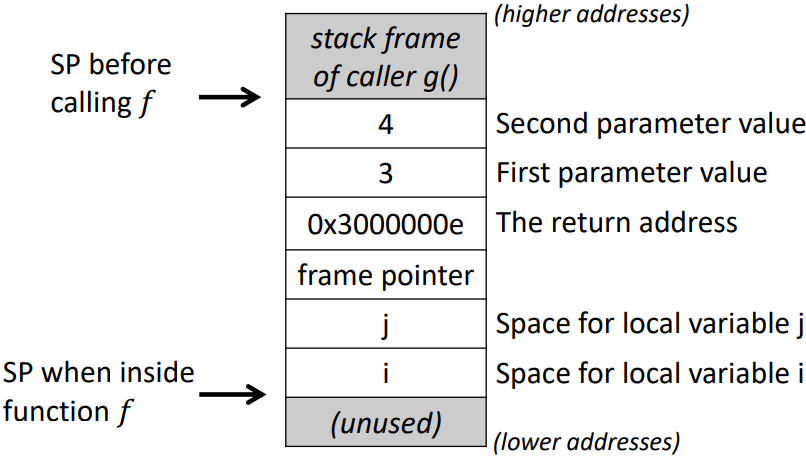
\includegraphics[width=0.45\textwidth,keepaspectratio]{stack_frame}
\end{figure}

\endgroup

\chapter{Buffer Overflows}

\section{Attack}

In C, the length of a string is not stored nor checked during runtime. Hence, writing a string with \ctext{lightGray}{strcpy} that is longer than its destination buffer will overwrite whatever comes after. 

Combined with the fact that C does not do any runtime check, it is possible to overwrite the stack frame with a buffer overflow. This means that it is possible to write a string containing the binary for the machine instructions for the function call, hence executing injected code.

Thanks to virtual memory, every process starts in a clean virtual address space with predictable addresses for the code \& the stack, hence it is easy for the attacker to know at which address the buffer will be located (\ctext{lightGray}{0xFFFFCEF} if function \ctext{lightGray}{f()} called from \ctext{lightGray}{main()}).

Buffer overflow attacks can be used to start a shell were the attacker can execute programs with the same rights as the attacked process.

\section{Protection}

\begin{itemize}
    \item \textblue{Avoid the attack} : use language like \textit{Java} or \textit{C\#} that checks the array lengths. In C, do not use \ctext{lightGray}{strcpy} (or \ctext{lightGray}{gets} and \ctext{lightGray}{sprintf}) but instead use \ctext{lightGray}{strncpy} or \ctext{lightGray}{snprintf}.
    \item \textblue{Allways check and sanitize data coming from outside} : verify that integers are nonnegative if they have to be, ...
    \item \textblue{Adding bound checking in C} : put \textit{guard pages} around the arry to tell the OS to raise an exception if somebody tries to access them (resource consuming)
    \item \textblue{Static analysis} of the source code to find vulnerabilities, use \textblue{fuzzers} to test the program with random inputs
    \item \textblue{Mitigation by Canaries} : push a random amount (so that it is unknown by the attacker) of \textit{canary bytes} (= data) onto the stack. When the function returns, it checks whether the canary value has been overwritten.
        \begin{itemize}
            \item This can fails if the attacer guesses the size of the random canary, it does not protect local variables (attacker can overwrite a function pointer variable to let it point to own code), and it makes the program slightly slower.
        \end{itemize}
    \item Make address of stack less predictable with \textblue{Address Space Layout Randomization (ASLR)} (add random offset). Might not work well on CPUs with a small address space (16-bits or 32-bits) and the attacker can succeeed by preparing large areas of memory on the heap if the randomization is not large enough.
        \begin{itemize}
            \item If the randomization is not larhe enought, the attacker can succeed by preparing large areas of memory on the heap, hoping that program execution will arrive there (\textit{heap spraying} : making lots of copies of his code to hope to fall on the right place in memory)
        \end{itemize}
    \item \textblue{Data Execution Prevention (DEP)} : most OS mark the memory pages where the stack is located as "\textit{not executable}"
        \begin{itemize}
            \item An attack can however still be successfull if we do not write our own attack code that already exists in the system, such as the \ctext{lightGray}{system("/bin/bash")} library function, used to start a shell. Calling this without writing you own code is possible : if ASLR is not used, library functions like system ones are located at predictable addresses. This is called \textit{Return Oriented Programming}.
        \end{itemize}
    \item \textblue{Mitigation} : 
        \begin{itemize}
            \item Check input data coming from outside
            \item Consider using a modern programming language
            \item Isolate your server from the rest of the system, to minimize the damage
            \item Do not run your web server as root
        \end{itemize}
\end{itemize}

\chapter{SQL Injection}

An SQL injection can happen whenever a system does not verify/sanitize user input. It is therefore used to perform unintended operations on a database like :
\begin{itemize}
    \item Bypass authentication mechanisms
    \item Read unavailable information from the database
    \item Write information such as new user accounts to the database
\end{itemize}

Example of how to perform SQL injections in 5 steps :
\begin{enumerate}
    \item \textblue{Make a guess on hpow the server works internally} : maybe the user accounts are stored in a database, think about what the authentication code should look like, probably something like \ctext{lightGray}{"SELECT name,} \ctext{lightGray}{pwd FROM users WHERE name='"+n+"'";}", with \ctext{lightGray}{n} being the user input.
    \item \textblue{Check if the system accepts unsanitized inputs} (e.g. put \ctext{lightGray}{steve@unixwiz.net} in the email field (wrong format)). If the server responds with an error, it did not filter the user input properly. One can also enter something like \ctext{lightGray}{anything' OR 'x'='x} in the email field, which makes the SQL query look like \ctext{lightGray}{SELECT fieldlist FROM table WHERE field = 'anything' OR 'x'='x';}, which return every item in the table.
    \item \textblue{Schema field mapping} : involves guessing the names of the columns, with inputs like \ctext{lightGray}{x' AND email IS NULL;--}, which returns an error if the guess is wrong.
    \item \textblue{Finding the table name} : \ctext{lightGray}{x' AND 1=(SELECT COUNT(*) FROM SomeGuessedTableName); --}
    \item \textblue{Creating a new user account} \ctext{lightGray}{x'; INSERT INTO users ('email', 'passwd', 'login\_id', 'name') VALUES ('steve@unixwiz.net', 'hello', 'steve', 'Steve Friedl'); --}. This step can go wrong for many reasons (not enough room in web form, no \textit{INSERT} permission on the users table, there might be other fields in the users table, ...)
        \begin{itemize}
            \item Alternative : modify an existing user : \ctext{lightGray}{x'; UPDATE users SET email = 'attacker@gmail.com'} \ctext{lightGray}{WHERE email = 'bob@example.com} (even better is the modified user is an admin)
        \end{itemize}
\end{enumerate}

Another possible inejction is the timing attacks are also possible to get the password of someone when \ctext{lightGray}{INSERT} and \ctext{lightGray}{UPDATE} are unavailable. The main idea is to get information on the password based on the time that the server makes to respond at a given query.

\ctext{lightGray}{x; SELECT IF(SUBSTRING(passwd,1,1) = CHAR(65), BENCHMARK(5000000,ENCODE('MSG','by 5 seconds')),null) FROM users WHERE name='Bob';}

If the server takes longer than usual to response the above query, we know that the first character of the password is \ctext{lightGray}{CHAR(65)}, i.e. 'A'.

Other injections also exist, for example select a background picture stored on the server, modifiy the cookie value to the directory were passwords are stores, etc.

\section{Mitigation}

\begin{itemize}
    \item Never trust data coming from outside : sanitize the input (no harmful characters)
    \item Use SQL prepared statements or stored procedures (query stored in the database as a procedure that can be called from the application, e.g. : \ctext{lightGray}{String query = "SELECT name,passwd FROM users WHERE name=?";} (Java))
    \item Limit database permissions
    \item Isolate the web server (use a DMZ)
    \item Configure error reporting : do not disclose more information than necessary
\end{itemize}

\chapter{Cross-Site Scriptin}

\textblue{Idea} : manipulate a user session when they are logged in.

HTTP does not know sessions (HTTP requests are stateless). The typical way to implement session in web applications is :
\begin{enumerate}
    \item Client (web browser) sends request to special URI with password
    \item Server verifies credentials and includes a session token in the header of the response to the client
    \item The token is stored as cookies in the browser, which will now include this cookie value in every request to the server
\end{enumerate}

\textblue{Naive approach} : put a link to our website in a review. When somebody clicks on it, our malicious code reads the user's session cookie.

\textblue{Same-origin policy} : prevents that JavaScript code in a open web page $X$ can access the data of another web page $Y$, by comparing the origin (host, port, protocol).

\section{Cross-site scripting (XSS)}

Insert JavaScript code into another web page. How to steal a cookie ?

\begin{itemize}
    \item Imagine a search engine where you enter your query in a \ctext{lightGray}{<search>} field, that is then sent to the server \ctext{lightGray}{http://www.find.com/search.php?query=UCL}. The server responds with a page that contain the search results and the search terms
    \item Code can be injected by entering search queries of the form \ctext{lightGray}{<script>some javascript</script>} if there is no sanitazation. In this case, the browser will execute the code
    \item Since it is running in the same context, it can access its cookies and execute scripts with privileges of the site (e.g. : send the content of the session token cookie to a server controlled by the attacker)
\end{itemize}

We just have to convince the user to open the manipulated links, e.g. by social engineering (spam mails, forum posts, chat messages, ..)

\textblue{Other examples} : web bases mail clients (put code into mail subject or body and victim reads mail in web browser)

There are two types of XSS :
\begin{itemize}
    \item \textblue{Reflected (non-persistent) XSS} : URLs (client-side), only affects result page of the search query
    \item \textblue{Stored (persistent) XSS} : Stored on the server (blog, chat, ...), inject code permanently on the server
\end{itemize}

\section{Mitigation}

\subsection{Server side}

\begin{itemize}
    \item Validate input, filter out HTML tags (sanitazation)
    \item Combine session cookies with client IP address
    \item Use special tools to check websites for vulnerabilities
\end{itemize}

\subsection{Client side}

\begin{itemize}
    \item Disable JavaScript
    \item Browsers contain XSS filters that check server responses for suspicious code
\end{itemize}

\section{Cross-side request forgery}

\textblue{Goal} : make a user request for us (i.e. by clicking a link to make a bank transfer and since the browser includes automatically the user cookie, it will be accepted)

\begin{enumerate}
    \item User $A$ logins to bank website $B$
    \item In a different window, user visits a chat forum $Y$
    \item Attacker $B$ inject XSS into $Y$ to manipulate $X$ (e.g. \ctext{lightGray}{<img src="http://X.com/transfer?account=A\& amount=10000\&to=B">})
    \item The browser will automatically include X.com's cookies in the requests and the query will be accepted $\rightarrow$ attacker \textit{rides} on the session of a different website
\end{enumerate}

Modern browsers inform a web server from which web page the request was sent.

\chapter{Network Scans}

Scans are information gathering attacks. The goal is to find vulnerabilities on hosts, discover network topology, system fingerprinting, ...

\section{Ping Sweeps}

The msot simple form of network scan. It is performed by sending ICMP echo requests :
\begin{itemize}
    \item If you get a reply, you know that there is someone at this address
    \item If you get \textit{host unreachable}, then nobody is there (or the access is blocked)
\end{itemize}

However, it is simple but unreliable as most sysadmins configure hosts to ignore/block ICMP echo packets.

\section{TCP Port Scans}

\begin{minipage}[t]{0.45\textwidth}
    \subsection{TCP With Regular Connection}
    Easy to implement but slow and resources consuming
	\begin{figure}[H]
		\centering
		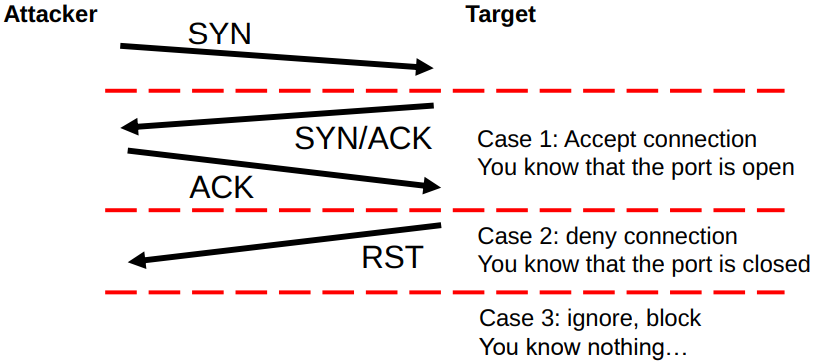
\includegraphics[width=\textwidth,keepaspectratio]{tcp_scan}
	\end{figure}
\end{minipage}
\hfill
\begin{minipage}[t]{0.45\textwidth}
    \subsection{TCP With SYN Only}
    Fast but not supported by the OS (you have to write your own code)
	\begin{figure}[H]
		\centering
		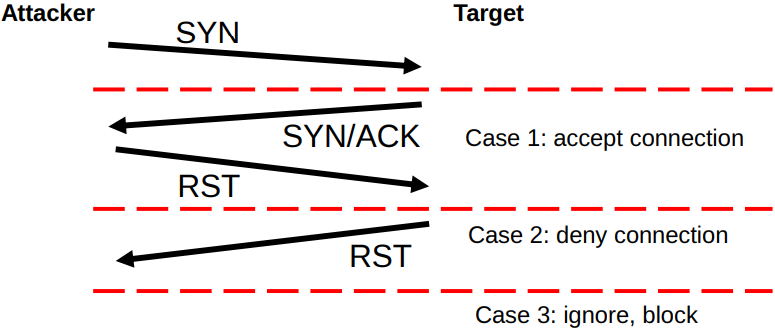
\includegraphics[width=\textwidth,keepaspectratio]{tcp_syn}
	\end{figure}
\end{minipage}

\subsection{TCP XMas-Tree Scan}

\begin{figure}[H]
    \centering
    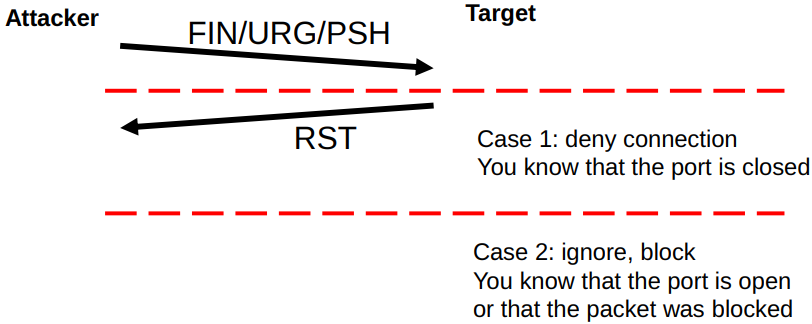
\includegraphics[width=0.5\textwidth,keepaspectratio]{tcp_xmas}
\end{figure}

\section{UDP Port Scan}

UPD is connectionless so the TCP approach does not work. We need to send a packet to the target and :
\begin{itemize}
    \item wait for a negative answer (i.e. '\textit{port unreachable}' ICMP message if UDP port is closed)
    \item wait for a positive answer
\end{itemize}

Easy to implement but not very reliable since UDP packets might be lost or ICMP might be diabled.

\section{Scan Types}

3 main types :
\begin{itemize}
    \item \textblue{Vertical scans} : scan all ports of a target
    \item \textblue{Horizontal scans} : find targets with open ports of interest
    \item \textblue{Block scans} : combinaison of both
\end{itemize}

\section{Obfuscation}

Scans are also possible for other protocla such as HTTP, smart home automation, ...

Scans might look suspicious for the cybersecurity engineer monitoring the traffic. There are solutions to obfuscate such footprinitng such as \textit{slow scan, distributed scan, indirect scan, ...}

\subsection{Idle scan}

The goal is to impersonate another computer whose network traffic is very slow or nonexistent (hides our address IP as attacker).

It is based on the fact that you can spoof the source IP address in the RCP header of a packer. The target server will therefore respond with a 'SYN/ACK' to the 'zombie' IP which will return a 'RST' containing a 'RST ID' that is sometimes just incremented by 1 each time. We only need to continuously ask the zombie to get a 'RST' in order to see a jump in the IDs

\begin{figure}[H]
    \centering
    \includegraphics[width=0.7\textwidth,keepaspectratio]{idlescan}
\end{figure}

\chapter{Denial Of Service (DoS)}

\textblue{Goal} : overload or crash a server to make the service unavailable to legitimate users.

\section{Types of DoS attacks}

\begin{itemize}
    \item \textblue{Semantic attacks} : make the server non functional by sending requests (e.g. :: sending queries that need a lot of time, that trigger errors, send half a request such that the server will keep the connection open, ... It is cheap for the attacker but requires specific knowledge of the target
    \item \textblue{Brute-force attacks} : overwhelm the server by sending many requests. If coodinated from multiple hosts, we say that it is a Distributed Denial Of Service (DDoS) 
    \item \textblue{Reflected DoS attacks} : same as DDoS but hides the attacker's IP address with spoofing (DRDoS, uses DNS). Leads to \textit{amplification} : the respoinse is larger that the request (solves the bandwidth problem for the attacekr, since DNS queries are very small (80B) and answer can go up to 400MB)
\end{itemize}

DNS servers are very popular for such attacks because they are open to anybody, they use UDP (perfect for spoofing) and they are made to handle high loads (high computational power).

\section{Mitigation}

\begin{itemize}
    \item Do not let open services that can be misused for DRDoS attacks (switch off unused services, etc. Note that it cannot be done for DRDoS attacks using DNS)
    \item Implement ingress filtering against reflective attacks : router discards packets if source IP does not match network address
\end{itemize}

\section{SYN flooding}

Host $A$ sends many SYN packets to host $B$. It consumes memory in $B$ because the OS allocated data structures for the assumed TCP connections that are not completed. 

$\rightarrow$ Protection with the TCPv4 header \& \textblue{SYN cookies} : $B$ does not allocate memory for the connection before receiving ACK packet from $A$. This ACK packet contains an ACK number, if the cookie is okay and not too old, it is very likely that $A$ sent a SYN before.

\chapter{Domain Name System (DNS)}

%TODO
